\documentclass[12pt]{article}\pagestyle{myheadings}
\usepackage{graphicx}
\usepackage{placeins}

\textwidth 7.0 truein
\oddsidemargin -0.25in   %left-hand edge
\evensidemargin -0.5 truein  %right-hand edge
\topmargin -0.85in      %top of paper to top of head, pulls whole unit
\textheight 9.5in

%Enter your last name, the portfolio problem number, and the draft number.
\title{Project 1: Non-adiabatic Explosion \\ Intermediate Numerical Analysis 1}
\author{Ian Char, Denis Kazakov, Evan Sidrow}
\date{December 1, 2015}


\usepackage{amsmath,amssymb,amsthm,amsfonts,graphicx}
%The following commands allow us to typeset theorems, propositions, definitions, etc.
\theoremstyle{plain}
\newtheorem{theorem}{Theorem}
\newtheorem{lemma}[theorem]{Lemma}
\newtheorem{corollary}[theorem]{Corollary}
\newtheorem{proposition}[theorem]{Proposition}
\newtheorem*{definition}{Definition}

\renewcommand{\qedsymbol}{\ensuremath{\blacksquare}}
\newcommand{\N}{\mathbb{N}}
\newcommand{\Z}{\mathbb{Z}}
\newcommand{\Q}{\mathbb{Q}}
\newcommand{\R}{\mathbb{R}}
\newcommand{\C}{\mathbb{C}} 

\begin{document}
\maketitle
\section{Overview}

\subsection{Introduction}
Throughout this project we consider a scenario in which fuel and oxidizer have been put into a container with temperature $T$. Although there is no immediate explosion, as the activation energy of this reaction is high, there are still some reactions occurring inside of the container that slowly begin to raise the internal temperature of the container. If the container is insulated well and heat accumulates much faster than it is lost to the environment, the heat from the initial few reactions will build up to cause an explosion. On the other hand, if sufficient amount of heat escapes from the box, heat loss will equal heat accumulation at some point and there will never be sufficient energy to cause an explosion (this is referred to as a fizzle). The goal of the project is to model both scenarios: an explosion and a fizzle.

\subsection{Physical Understanding}
Let $A$ be the current amount of fuel in the container. The rate that the fuel is used up is described by $(\ref{eq:changeFuel})$.

\begin{equation}\label{eq:changeFuel}
\frac{dA}{dt} = -\bar{c} A e^{-E/RT}
\end{equation}
Here, $\bar{c}$ is a constant of proportionality, $E$ is the activation energy for the reaction, $R$ is the universal gas constant, and $T$ is the current temperature inside of the container. Therefore, $e^{-E/RT}$ is related to the proportion of fuel molecules which have sufficient energy to overcome the high activation energy and react with the oxidizer. Another assumption that we can take advantage of is that thermal energy is conserved in the system. 

\begin{equation}\label{eq:consEnergy}
\frac{dU}{dt} = Q + W
\end{equation}

In $(\ref{eq:consEnergy})$, $\frac{dU}{dt}$ is the change in thermal energy inside of the container, $Q$ is the thermal energy generated inside the container, and $W$ is the thermal energy lost due to some amount of work (this term is 0 for this scenario). To yield a useful result, we substitute values in for $(\ref{eq:consEnergy})$. The change in energy is equal to $c_{v} \frac{dT}{dt}$, where $c_{v}$ is the heat capacity at constant volume. From $(\ref{eq:changeFuel})$, the amount of heat being generated is $- \bar{c} \frac{dA}{dt}$, and the heat being lost to outside of the box is $-h (T - T_{0})$ where $h$ is a parameter indicating the amount of insulation in the container and $T_{0}$ is the initial temperature inside of the container. Putting this all together we get the following.

\begin{equation}\label{eq:physEqn}
c_{v} \frac{dT}{dt} = - \bar{c} \frac{dA}{dt} -h (T - T_{0})
\end{equation}

\subsection{Non-dimensionalizing the Problem}
In order to make $(\ref{eq:physEqn})$ easier to solve numerically we non-dimensionalize it. First we define $\delta$, which is proportional to $\frac{1}{h}$. For time we define $\sigma = \frac{t}{\delta t_{ref}}$, where $t_{ref}$ is a reference time which represents the soonest possible explosion time (if the container is perfectly insulated, so $\delta \rightarrow \infty$). For temperature we define $\bar{T} = \frac{T}{T_{0}} = 1 + \epsilon \theta$ where $\epsilon = \frac{RT_{0}}{E}$. Notice that at the beginning of the problem $\epsilon$ will be very small because the activation energy will be much higher than the amount of energy currently in the system. Using the following definitions we get the following.

\begin{equation}\label{eq:nonDEq}
\frac{d\theta}{d\sigma} = \delta e^{\theta} - \theta
\end{equation}

The initial condition of this problem is $\theta(0) = 0$, where $\theta$ is a function of $\sigma$. This makes sense, as $\theta$ represents a change in thermal energy compared to the initial state, and $\sigma$ represents a proportion of time compared to a reference time. It is also important to note that although the problem is now non-dimensionalized, the physical implications can still be observed: $\frac{d\theta}{d\sigma}$ represents the change in energy of the system, $\delta e^{\theta}$ represents the energy being generated in the system by the reaction, and $\theta$ represents the energy being lost to the environment.

\vspace{5mm}

Using $(\ref{eq:nonDEq})$, we can also find the dividing value of $\delta$ that separates cases where the reaction fizzles and where the reaction explodes. To do this we first note that we must have values of  $\delta$ and $\theta$ that satisfies $\delta e^{\theta} - \theta = 0$. However, since we are looking for the boundary between a fizzle and explosion (the osculation point), the values must also satisfy $\frac{d}{d\theta}\left(\delta e^{\theta} \right) = \frac{d}{d\theta}\left(\theta \right)$. Using the two equations we find that $\theta_{div} = 1$ and $\delta_{div} = 1/e$. Thus, all values of $\delta$ less than $1/e$ fizzle while all values greater than $1/e$ explode.

\section{A Fizzle Reaction}
\subsection{Numerical Integration of the ODE}
We first consider the case in which $\delta = \frac{1}{5}$. Already it is known that this will cause the system to fizzle rather than explode because $\delta < \frac{1}{e}$. Although there is no way to find a closed form of the solution, the behavior of the solution can be modeled through numerical integration. To integrate the ODE, 4th order Runge-Kutta can be used with a step size of $h = 10^{-3}$. Because this is a fizzle case, it is known that the solution will eventually converge to some $\theta_{fizzle}$. As such, the numerical integration process will run until the change in $\theta$ is less than a tolerance of $10^{-6}$. The first 10 steps and last 10 steps of the integration are displayed in Table 1 (for display purposes, all numbers have been rounded to the nearest $10^{-7}$ value).

\begin{table}[ht!]
\centering
\begin{tabular} {| l | l | l | l | l | l |}
\hline
$\sigma$ & $\theta$ & $k_{1}$ & $k_{2}$ & $k_{3}$ & $k_{4}$ \\
\hline
0.0 & 0.0 & 0.0002 & 0.0001999 & 0.0001999 & 0.0001998 \\
0.001 & 0.0001999 & 0.0001998 & 0.0001998 & 0.0001998 & 0.0001997 \\
0.002 & 0.0003997 & 0.0001997 & 0.0001996 & 0.0001996 & 0.0001995 \\
0.003 & 0.0005993 & 0.0001995 & 0.0001994 & 0.0001994 & 0.0001994 \\
0.004 & 0.0007987 & 0.0001994 & 0.0001993 & 0.0001993 & 0.0001992 \\
0.005 & 0.0009980 & 0.0001992 & 0.0001991 & 0.0001991 & 0.0001990 \\
0.006 & 0.0011971 & 0.0001990 & 0.0001990 & 0.0001990 & 0.0001989 \\
0.007 & 0.0013961 & 0.0001989 & 0.0001988 & 0.0001988 & 0.0001987 \\
0.008 & 0.0015949 & 0.0001987 & 0.0001986 & 0.0001986 & 0.0001986 \\
0.009 & 0.0017935 & 0.0001986 & 0.0001985 & 0.0001985 & 0.0001984 \\
... & ... & ... & ... & ... & ... \\
7.031 & 0.2578126 & 1e-06 & 1e-06 & 1e-06 & 1e-06 \\
7.032 & 0.2578136 & 1e-06 & 1e-06 & 1e-06 & 1e-06 \\
7.033 & 0.2578146 & 1e-06 & 1e-06 & 1e-06 & 1e-06 \\
7.034 & 0.2578156 & 1e-06 & 1e-06 & 1e-06 & 1e-06 \\
7.035 & 0.2578166 & 1e-06 & 1e-06 & 1e-06 & 1e-06 \\
7.036 & 0.2578176 & 1e-06 & 1e-06 & 1e-06 & 1e-06 \\
7.037 & 0.2578186 & 1e-06 & 1e-06 & 1e-06 & 1e-06 \\
7.038 & 0.2578196 & 1e-06 & 1e-06 & 1e-06 & 1e-06 \\
7.039 & 0.2578206 & 1e-06 & 1e-06 & 1e-06 & 1e-06 \\
7.04 & 0.2578216 & 1e-06 & 1e-06 & 1e-06 & 1e-06 \\
\hline
\end{tabular}
\caption{The first 10 and last 10 steps of integration for $\delta = \frac{1}{5}$}
\end{table}

\break

\subsection{Late Solution}
One way that the previous solution can be checked is to compare it against the long-time solution of the problem. For this case, the late solution will just be the value that the system approaches. To find this value we set $\frac{d\theta}{d\sigma} = 0$. We are now faced with solving for values of $\theta_{fizzle}$ in the following equation.
\[\delta e^{\theta_{fizzle}} - \theta_{fizzle} = 0\]
The solution of this equation can be found using the secant method with initial guesses $\theta_{fizzle} = 0.1$ and $\theta_{fizzle} = 0.2$. Table 2 lists out the iterations needed until the relative change in $\theta_{fizzle}$ is less than $10^{-3}$.

\begin{table}[ht!]
\centering
\begin{tabular} {| l | l | l | l | l | l |}
\hline
Iteration Number & $\theta_{fizzle}$ \\
\hline
0 & 0.1 \\
1 & 0.2 \\
2 & 0.257691799708 \\
3 & 0.259156250269 \\
4 & 0.259171097979 \\
\hline
\end{tabular}
\caption{The iterations required to converge on $\theta_{fizzle}$}
\end{table}

Although $\theta_{fizzle}$ does not match the value converged upon in Table 1, the similarity between the two shows that the integration of the ODE is fairly accurate. Furthermore, it is likely that if $\sigma$ were to be expanded beyond $\sigma = 7.04$ then the value would be even closer to $\theta_{fizzle}$. 

\subsection{Early Solution}

In addition, a short-time solution can be found to confirm that the initial steps of the numerical integration are correct. To find this, we first start with expanding $\delta e^{\theta}$ into a Taylor series. 
\[\frac{d\theta}{d\sigma} = \delta \left(1 + \theta + \frac{\theta^{2}}{2!} + \frac{\theta^{3}}{3!} + ...\right) - \theta\]
Taking the first two terms of the Taylor series, the following approximation can be made.
\[\frac{d\theta}{d\sigma}\approx \delta + \theta (\delta - 1)\] Unlike the original ODE, this ODE can be solved analytically via separation of variables. Doing so yields the following result. 
\begin{equation}\label{eq:appxEarly}
\theta \approx \left(\frac{\delta}{\delta - 1}\right) e^{(\delta - 1)\sigma} - \left(\frac{\delta}{\delta - 1}\right)
\end{equation}
Now that both an early and late solution have been obtained, the two solutions can be plotted along with the solution found with 4th order Runge-Kutta (Figure 1). Since the early and late solutions only describe the solution for certain periods of the overall reaction, each are plotted until the difference between the integrated solution and the approximation is greater than $10^{-3}$ in $\theta$.

\begin{figure}[h]
\centering
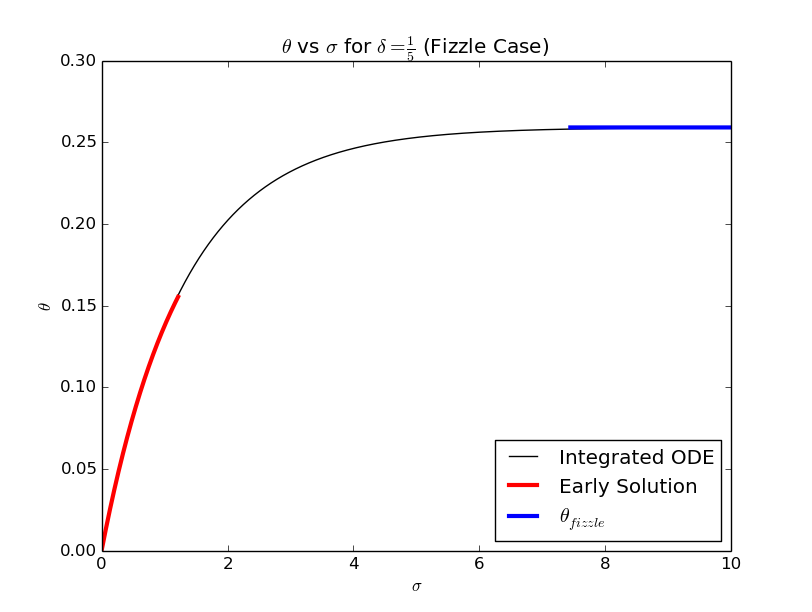
\includegraphics[scale=0.75]{Part1.png}
\caption{A plot of the integrated ODE, early solution, and late solution from $0 \le \sigma \le 10$ and where $\delta = \frac{1}{5}$}
\label{fig:Part1}
\end{figure}

Figure 1 provides a visual confirmation for the accuracy of the integrated ODE. The early and late solutions found seem to match the result produced by the 4th order Runge-Kutta remarkably well.

\subsection{Physical Implications}
From exploring the case where $\delta = \frac{1}{5}$, we can learn more about the nature of the reaction. First, recall the Taylor expansion of the ODE that was used when finding the early solution of the problem: 
\[\frac{d\theta}{d\sigma} = \delta \left(1 + \theta + \frac{\theta^{2}}{2!} + \frac{\theta^{3}}{3!} + ...\right) - \theta\]
Looking at this in a physical sense, we note that the left hand side represents the amount of heat being accumulated, $\delta \left(1 + \theta + \frac{\theta^{2}}{2!} + \frac{\theta^{3}}{3!} + ...\right)$ represents the heat being generated, and the $\theta$ term represents the heat being lost to outside the container. Since the problem starts with $\theta = 0$ and $\sigma = 0$, it is easy to make the assumption that the heat loss plays an insignificant role at the start of the problem since the heat being generated will be on the order of some constant while $\theta \ll 1$. In order to test this hypothesis, we assume that at the start of the problem the ODE can be approximated as the following.

\[\frac{d\theta}{d\sigma} \approx \delta e^{\theta}\]

This equation can then be solved using separation of variables.

\[\int e^{-\theta} d\theta \approx \delta \int d\sigma\]
\[-e^{-\theta} \approx \delta \sigma + c\]
\[\theta \approx ln\left(\frac{1}{\delta(c - \sigma)}\right)\]

Then using the initial conditions to solve for c...

\[0 = ln\left(\frac{1}{\delta c}\right) \quad \rightarrow \quad c = \frac{1}{\delta}\]
\begin{equation} \label{eq:fizzHeatLoss}
\theta \approx ln\left(\frac{1}{1 - \delta \sigma}\right)
\end{equation}
\begin{equation} \label{eq:fizzHeatGain}
\delta e^{\theta} \approx \frac{\delta}{1 - \delta \sigma}
\end{equation}

Relating this back to the original ODE, we see that the total heat being accumulated and the heat generation can be represented approximately with $(\ref{eq:fizzHeatGain})$ and the heat lost to the environment can be represented  approximately with $(\ref{eq:fizzHeatLoss})$. This conforms to the hypothesis that the heat loss is the least significant term at the beginning of the problem since for small $\sigma$ $(\ref{eq:fizzHeatLoss}) < (\ref{eq:fizzHeatGain})$. As a result, we see that at the beginning of the problem heat generation plays a much larger role than heat loss. On top of this, we know that in the late solution for a fizzle the amount of heat being generated is equal to the amount of heat being lost. Thus, while the heat loss to the environment starts out playing a relatively insignificant role in the beginning of the reaction, by the end of the reaction it has increased to match the amount of heat being generated. Therefore, the accumulation of energy is impeded before it can reach the required activation energy needed for an explosion.


\section{An Explosive Reaction}

\subsection{Numerical Integration of the ODE}

After looking at the fizzle reaction ($\delta = 1/5 < 1/e $), we now look to the explosive reaction, where $\delta = 1 > 1/e$, which corresponds to an explosive reaction. In this case, solving the differential equation {\[ \frac{d\sigma}{d\theta} = \frac{1}{\delta e^{\theta} - \theta} \]}in order to find $\sigma(\theta)$ is easier than solving the original differential equation. This is because an explosion results in a vertical asymptote in $\theta(\sigma)$, so the original equation is stiff and difficult to solve numerically. In order to find a numerical solution to this equation, Fourth-Order Runge-Kutta was used with a step size of $h = 10^{-3}$ and an initial condition $\sigma(0) = 0$, since at $\theta = 0$, the temperature of the box is by definition its initial temperature and at $\sigma = 0$, time is at its initial state. Since this is an explosion, it is known that there is a specific time of explosion which corresponds to a value of $\sigma = \sigma_{exp}$. Therefore, the numerical integration will take place until the change in $\sigma$ is less than $10^{-6}$, indicating that $\sigma \rightarrow \sigma_{exp}$. The first 10 steps and last 10 steps of the calculation are shown in the table below:

\begin{table}[ht!]
\centering
\begin{tabular} {| l | l | l | l | l | l |}
\hline
$\theta$ & $\sigma$ & $k_{1}$ & $k_{2}$ & $k_{3}$ & $k_{4}$ \\
\hline
0.0 & 0.0 & 0.001 & 0.0009999999 & 0.0009999999 & 0.0009999995 \\
0.001 & 0.0009999998 & 0.0009999995 & 0.0009999989 & 0.0009999989 & 0.0009999980 \\
0.002 & 0.0019999987 & 0.0009999980 & 0.0009999969 & 0.0009999969 & 0.0009999955 \\
0.003 & 0.0029999955 & 0.0009999955 & 0.0009999939 & 0.0009999939 & 0.0009999920 \\
0.004 & 0.0039999893 & 0.0009999920 & 0.0009999899 & 0.0009999899 & 0.0009999875 \\
0.005 & 0.0049999791 & 0.0009999875 & 0.0009999848 & 0.0009999848 & 0.0009999820 \\
0.006 & 0.0059999639 & 0.0009999820 & 0.0009999788 & 0.0009999788 & 0.0009999754 \\
0.007 & 0.0069999427 & 0.0009999754 & 0.0009999718 & 0.0009999718 & 0.0009999679 \\
0.008 & 0.0079999145 & 0.0009999679 & 0.0009999638 & 0.0009999638 & 0.0009999594 \\
0.009 & 0.0089998782 & 0.0009999594 & 0.0009999547 & 0.0009999547 & 0.0009999498 \\
... & ... & ... & ... & ... & ... \\
6.905 & 1.3580917773 & 1.0098e-06 & 1.0092e-06 & 1.0092e-06 & 1.0087e-06 \\
6.906 & 1.3580927866 & 1.0087e-06 & 1.0082e-06 & 1.0082e-06 & 1.0077e-06 \\
6.907 & 1.3580937948 & 1.0077e-06 & 1.0072e-06 & 1.0072e-06 & 1.0067e-06 \\
6.908 & 1.3580948020 & 1.0067e-06 & 1.0062e-06 & 1.0062e-06 & 1.0057e-06 \\
6.909 & 1.3580958082 & 1.0057e-06 & 1.0052e-06 & 1.0052e-06 & 1.0047e-06 \\
6.910 & 1.3580968134 & 1.0047e-06 & 1.0042e-06 & 1.0042e-06 & 1.0037e-06 \\
6.911 & 1.3580978176 & 1.0037e-06 & 1.0032e-06 & 1.0032e-06 & 1.0027e-06 \\
6.912 & 1.3580988208 & 1.0027e-06 & 1.0022e-06 & 1.0022e-06 & 1.0017e-06 \\
6.913 & 1.3580998229 & 1.0017e-06 & 1.0012e-06 & 1.0012e-06 & 1.0007e-06 \\
6.914 & 1.3581008241 & 1.0007e-06 & 1.0001e-06 & 1.0001e-06 & 0.9996e-06 \\
\hline
\end{tabular}
\caption{The first 10 and last 10 steps of integration for $\delta = 1$}
\end{table}

\subsection{Determination of the Time of Explosion}

In order to find the approximate time that the box explodes, we can integrate the differential equation from $\theta = 0$ to $\theta = \infty$ to find the value of $\sigma$ as $\theta$ approaches $\infty$, indicating an explosion. Therefore, the following equation gives the asympotitc value of $\sigma_{exp}$:

{\[\sigma_{exp} = \int_0^\infty \frac{dx}{\delta e^{x} - x} \]} In order to integrate, it is easier to work with finite limits of integration. Therefore, we introduce the transformation:

{\[x = \frac{t}{1-t}\]}
{\[dx = \frac{dt}{(1-t)^{2}}\]} and so:

{\[\sigma_{exp} = \int_0^1 \frac{dt}{(\delta e^{\frac{t}{1-t}} - \frac{t}{1-t})(1-t)^{2}} \]} and now this equation can be integrated using Simpson's composite three-eighths rule. Note that the function is undefined at t = 1, but the exponential term in the denominator is the fastest growing term and therefore the function approaches zero as t approaches 1. This was used in the numerical integration scheme. Since the number of divisions for Simpson's three-eighths rule must be a multiple of three, A step size of $h = \frac{0.01}{3}$ was used. The first 10 and last 10 steps of the calculation are shown below:

\begin{table}[ht!]
\centering
\begin{tabular} {| l | l | l | l | l | l |}
\hline
t & $f(t)$ \\
\hline
0.0000000000 & 1.0 \\
0.0033333333 & 1.006694512266 \\
0.0066666667 & 1.013444986352 \\
0.0100000000 & 1.020251826563 \\
0.0133333333 & 1.027115434829 \\
0.0166666667 & 1.034036210419 \\
0.0200000000 & 1.041014549654 \\
............ & .............. \\
0.9800000000 & 1.311e-18 \\
0.9833333333 & 8.569e-23 \\
0.9866666667 & 4.096e-29 \\
0.9900000000 & 1.011e-39 \\
0.9933333333 & 4.388e-61 \\
0.9966666667 & 1.259e-125 \\
1.0000000000 & 0.000 \\
\hline
\end{tabular}
\caption{The first 7 and last 7 steps of integration for Simpson's 3/8 rule}
\end{table} After using Simpson's composite 3/8 rule on the values from Table 4, it was determined that  $\sigma_{exp} \approx 1.3590983$. Since $\sigma_{exp} = \frac{t}{\delta t_{ref}}$, and $\delta = 1$, then:

{\[ t_{exp} \approx 1.3590983* t_{ref} \]} So the explosion when $\delta = 1$ takes place 0.3590983 times later than the case when the box is perfectly insulated, which is when $\delta \rightarrow \infty$.


\subsection{Long-Time Solution}

When the box is very close to exploding (i.e. $\theta$ is large), the linear term of $\theta$ in the denominator of the differential equation or the term which corresponds to heat loss from the box- can be ignored:

{\[ \frac{d\sigma}{d\theta} = \frac{1}{\delta e^{\theta} - \theta} \approx \frac{1}{\delta e^{\theta}} \]}

{\[ d\sigma \approx \frac{d\theta}{\delta e^{\theta}} \]}

{\[ \int_{\sigma}^{\sigma_{exp}} dt \approx \int_{\theta}^{\infty} \frac{dt}{\delta e^{t}} \]}

{\[ \sigma_{exp} - \sigma \approx \frac{1}{\delta e^{\theta}}\]}

{\[\sigma(\theta) \approx \sigma_{exp} - \frac{1}{\delta e^{\theta}}\]}

The equation above, then, is an approximation for the solution close to the explosion. A plot of this approximation can be seen in Section 3.5.

\subsection{Short-Time Solution}

($\ref{eq:appxEarly}$) can be used in the explosive case where $\delta = 1$:

\[\theta \approx \left(\frac{\delta}{\delta - 1}\right) \left(e^{(\delta - 1)\sigma} - 1\right)\] However, since this formula is undefined at $\delta = 1$, L'Hopital's rule must be used, yielding the following:

\[\lim_{\delta \rightarrow 1} \left(\frac{\delta}{\delta - 1}\right) \left(e^{(\delta - 1)\sigma} - 1\right) = \lim_{\delta \rightarrow 1} \delta\sigma e^{(\delta -1) \sigma} + e^{(\delta-1)\sigma} -1 = \sigma + 1  - 1 = \sigma \] Therefore, a short-time solution to the differential equation is:

{\[\theta(\sigma) \approx \sigma\]} or:
{\[\sigma(\theta) \approx \theta\]}

\subsection{Plot of Results}

The following figures show the solution of the ODE with $\delta = 1$. The first figure shows $\sigma$ versus $\theta$, and the second shows $\theta$  versus $\sigma$ to be consistent with the solution from Section 2.

It is important to note that the numerical solution to the ODE is plotted until the slope of the solution curve is less than $10^{-3}$. The early solution is plotted until the absolute error in $\theta$ is greater than 0.05, and the late solution is plotted until the absolute error in $\theta$ is greater than 0.01.

\begin{figure}[h]
\centering
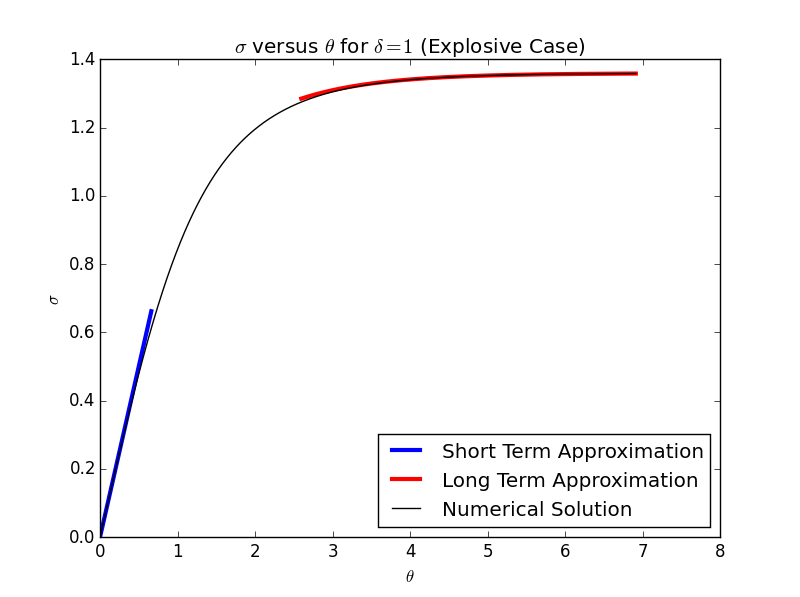
\includegraphics[scale=0.75]{sig_vs_th.png}
\caption{A plot of $\sigma$ vs $\theta$ for the integrated ODE, early solution, and late solution from $0 \le \theta \le 6.914$, where $\delta = 1$}
\label{fig:Part1}
\end{figure}

\begin{figure}[ht!]
\centering
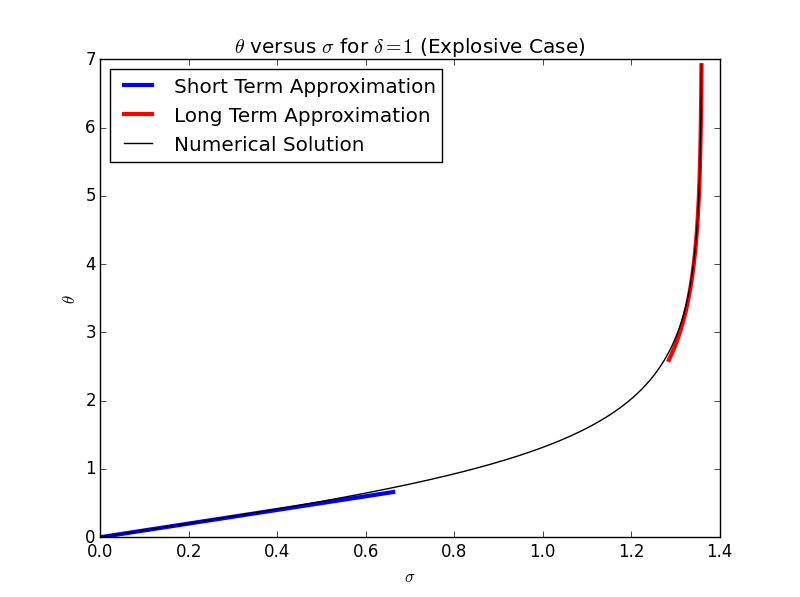
\includegraphics[scale=0.75]{th_vs_sig.png}
\caption{A plot of $\theta$ vs $\sigma$ for the integrated ODE, early solution, and late solution from $0 \le \sigma \le 1.359$, where $\delta = 1$}
\label{fig:Part1}
\end{figure}

\FloatBarrier

\subsection{Physical Implications}

In the case where $\delta = 1 > 1/e$, which results in an explosion, numerically solving the ODE gives insight into the physics of what is going on inside of the box.

In the short-term solution, using L'Hopital's rule gives that the relationship between $\theta$ and $\sigma$ is approximately linear initially. This is valid until $\sigma \approx 0.66$, which is where the numerical solution and the approximate short-term solution differ by more than 0.05 in $\theta$. The linear relationship means that the heat generation and heat loss terms of the solution are growing at the same rate when the reaction starts, or when $\theta = \sigma = 0$. This means that $\delta = 1$ is a sort of boundary. If $\delta < 1$, then the heat loss term is increasing faster than the heat generation term initially, meaning that the solution starts to level off initially before growing rapidly and exploding at $\sigma_{exp}$. In other words, the curve starts concave down. Of course, it will still explode eventually if $\delta > 1/e$, as the heat generation term will increase faster as time goes on and the heat loss term will never catch up. However, if $\delta > 1$, then the heat generation rate is always increasing faster than the heat loss rate, and the box always looks like it will explode, even initially. In other words, the solution curve is always concave up.

In the case of the long term solution, the primary conclusion to be drawn is that the heat loss term becomes utterly insignificant when the box is very close to exploding. To support this claim, consider that when assuming the following that the heat loss term is negligible, one can derive the following:

{\[\sigma(\theta) \approx \sigma_{exp} - \frac{1}{\delta e^{\theta}}\]}

{\[\delta e^{\theta} \approx \frac{1}{\sigma_{exp} - \sigma}\]}

{\[\theta \approx ln\left(\frac{1}{\delta(\sigma_{exp} - \sigma)}\right)\]}

Note that when the box is close to exploding, $\delta(\sigma_{exp} - \sigma) = \sigma_{exp} - \sigma$ is small, so then $\frac{1}{(\sigma_{exp} - \sigma)} \approx \delta e^{\theta}$ (the heat generation term) is large. Any large number is much larger than its natural logarithm, and in this case $ln\left(\frac{1}{\sigma_{exp} - \sigma}\right) \approx \theta$ (the heat loss term). Therefore, it is fair to assume that the heat loss term is negligible when $\sigma$ is close to $\sigma_{exp}$. In particular, this assumption is valid after $\sigma \approx 1.28$ (remember that $\sigma_{exp} \approx 1.359$), as this is where the long term approximation and numerical solution begin to agree within 0.01 of each other in $\theta$.

\section{Conclusion}
Through the numerical solutions that have been performed throughout this lab, we are able to get an insight to the physical nature behind this problem. After numerically integrating each case of the reaction ($\delta = 1/5$ and $\delta = 1$) we were able to see how the reaction evolved over time. We learned even more by creating approximations for the early and late stages of the problem. Near the beginning of the problem it was found that the heat generation ($Q_{gen}$) dominated the amount of heat lost to the environment ($Q_{loss}$). However, as the problem progresses the amount of $Q_{loss}$ starts to increase. Whether $Q_{loss}$ ever catches up to the magnitude of $Q_{gen}$ dictates the nature of the problem. If $\delta < 1/e$, $Q_{loss}$ catches up to $Q_{gen}$ and there is a fizzle, whereas if $\delta > 1/e$ the $Q_{loss}$ never catches up and there is an explosion. This in turn dictates the nature of the reaction because if $Q_{loss}$ is allowed to catch up to the magnitude of $Q_{gen}$, the system will be fixed at some amount of energy as heat loss and heat generation are in equilibrium. On the other hand, when $Q_{loss}$ never catches up, the total heat of the system is allowed to grow exponentially and overcome the large activation energy required to start the explosion. Overall, we were able to explore how both heat loss and generation of the system behave to create either a fizzle or explosion in a container.
\end{document}